\chapter{動態規劃}


\section{Triangle} %%%%%%%%%%%%%%%%%%%%%%%%%%%%%%
\label{sec:triangle}


\subsubsection{描述}
Given a triangle, find the minimum path sum from top to bottom. Each step you may move to adjacent numbers on the row below.

For example, given the following triangle
\begin{Code}
[
     [2],
    [3,4],
   [6,5,7],
  [4,1,8,3]
]
\end{Code}
The minimum path sum from top to bottom is 11 (i.e., 2 + 3 + 5 + 1 = 11).

Note: Bonus point if you are able to do this using only $O(n)$ extra space, where n is the total number of rows in the triangle.


\subsubsection{分析}
設狀態為$f(i, j)$,表示從從位置$(i,j)$出發,路徑的最小和,則狀態轉移方程為
$$
f(i,j)=\min\left\{f(i+1,j),f(i+1,j+1)\right\}+(i,j)
$$


\subsubsection{代碼}
\begin{Code}
// LeetCode, Triangle
// 時間複雜度O(n^2),空間複雜度O(1)
class Solution {
public:
    int minimumTotal (vector<vector<int>>& triangle) {
        for (int i = triangle.size() - 2; i >= 0; --i)
            for (int j = 0; j < i + 1; ++j)
                triangle[i][j] += min(triangle[i + 1][j],
                        triangle[i + 1][j + 1]);

        return triangle [0][0];
    }
};
\end{Code}


\subsubsection{相關題目}
\begindot
\item 無
\myenddot


\section{Maximum Subarray} %%%%%%%%%%%%%%%%%%%%%%%%%%%%%%
\label{sec:maximum-subarray}


\subsubsection{描述}
Find the contiguous subarray within an array (containing at least one number) which has the largest sum.

For example, given the array \code{\[−2,1,−3,4,−1,2,1,−5,4\]},
the contiguous subarray \code{\[4,−1,2,1\]} has the largest \code{sum = 6}.


\subsubsection{分析}
最大連續子序列和,非常經典的題。

當我們從頭到尾遍歷這個數組的時候,對於數組裏的一個整數,它有幾種選擇呢?它只有兩種選擇: 1、加入之前的SubArray;2. 自己另起一個SubArray。那什麼時候會出現這兩種情況呢?

如果之前SubArray的總體和大於0的話,我們認為其對後續結果是有貢獻的。這種情況下我們選擇加入之前的SubArray

如果之前SubArray的總體和為0或者小於0的話,我們認為其對後續結果是沒有貢獻,甚至是有害的(小於0時)。這種情況下我們選擇以這個數字開始,另起一個SubArray。

設狀態為\fn{f[j]},表示以\fn{S[j]}結尾的最大連續子序列和,則狀態轉移方程如下:
\begin{eqnarray}
f[j] &=& \max\left\{f[j-1]+S[j],S[j]\right\}, \text{ 其中 }1 \leq j \leq n \nonumber \\
target &=& \max\left\{f[j]\right\}, \text{ 其中 }1 \leq j \leq n \nonumber
\end{eqnarray}

解釋如下:
\begindot
\item 情況一,S[j]不獨立,與前面的某些數組成一個連續子序列,則最大連續子序列和為$f[j-1]+S[j]$。
\item 情況二,S[j]獨立劃分成為一段,即連續子序列僅包含一個數S[j],則最大連續子序列和為$S[j]$。
\myenddot  

其他思路:
\begindot
\item 思路2:直接在i到j之間暴力枚舉,複雜度是$O(n^3)$
\item 思路3:處理後枚舉,連續子序列的和等於兩個前綴和之差,複雜度$O(n^2)$。
\item 思路4:分治法,把序列分為兩段,分別求最大連續子序列和,然後歸併,複雜度$O(n\log n)$
\item 思路5:把思路2$O(n^2)$的代碼稍作處理,得到$O(n)$的算法
\item 思路6:當成M=1的最大M子段和
\myenddot


\subsubsection{動規}
\begin{Code}
// LeetCode, Maximum Subarray
// 時間複雜度O(n),空間複雜度O(1)
class Solution {
public:
    int maxSubArray(vector<int>& nums) {
        int result = INT_MIN, f = 0;
        for (int i = 0; i < nums.size(); ++i) {
            f = max(f + nums[i], nums[i]);
            result = max(result, f);
        }
        return result;
    }
};
\end{Code}


\subsubsection{思路5}
\begin{Code}
// LeetCode, Maximum Subarray
// 時間複雜度O(n),空間複雜度O(n)
class Solution {
public:
    int maxSubArray(vector<int>& A) {
        return mcss(A.begin(), A.end());
    }
private:
    // 思路5,求最大連續子序列和
    template <typename Iter>
    static int mcss(Iter begin, Iter end) {
        int result, cur_min;
        const int n = distance(begin, end);
        int *sum = new int[n + 1];  // 前n項和

        sum[0] = 0;
        result = INT_MIN;
        cur_min = sum[0];
        for (int i = 1; i <= n; i++) {
            sum[i] = sum[i - 1] + *(begin  + i - 1);
        }
        for (int i = 1; i <= n; i++) {
            result = max(result, sum[i] - cur_min);
            cur_min = min(cur_min, sum[i]);
        }
        delete[] sum;
        return result;
    }
};
\end{Code}


\subsubsection{相關題目}
\begindot
\item Binary Tree Maximum Path Sum,見 \S \ref{sec:binary-tree-maximum-path-sum}
\myenddot


\section{Palindrome Partitioning II} %%%%%%%%%%%%%%%%%%%%%%%%%%%%%%
\label{sec:palindrome-partitioning-ii}


\subsubsection{描述}
Given a string s, partition s such that every substring of the partition is a palindrome.

Return the minimum cuts needed for a palindrome partitioning of s.

For example, given \code{s = "aab"},

Return 1 since the palindrome partitioning \code{\["aa","b"\]} could be produced using 1 cut.

Reference \myurl{https://www.youtube.com/watch?v=lDYIvtBVmgo}


\subsubsection{分析}
定義狀態\fn{f(i,j)}表示區間\fn{[i,j]}之間最小的cut數,則狀態轉移方程為 
$$
f(i,j)=\min\left\{f(i,k)+f(k+1,j)\right\}, i \leq k \leq j, 0 \leq i \leq j<n
$$
這是一個二維函數,實際寫代碼比較麻煩。
 
所以要轉換成一維DP。如果每次,從i往右掃描,每找到一個迴文就算一次DP的話,就可以轉換為\code{f(i)=區間[i, n-1]之間最小的cut數},n為字符串長度,則狀態轉移方程為
$$
f(i)=\min\left\{f(j+1)+1\right\}, i \leq j<n
$$

一個問題出現了,就是如何判斷\fn{[i,j]}是否是迴文?每次都從i到j比較一遍?太浪費了,這裏也是一個DP問題。

定義狀態\fn{P[i][j] = true if [i,j]為迴文},那麼
\begin{Code}
P[i][j] = str[i] == str[j] && P[i+1][j-1]
\end{Code}


\subsubsection{代碼}
\begin{Code}
// LeetCode, Palindrome Partitioning II
// 時間複雜度O(n^2),空間複雜度O(n^2)
class Solution {
public:
    int minCut(const string& s) {
        const int n = s.size();
        int f[n+1];
        bool p[n][n];
        fill_n(&p[0][0], n * n, false);
        //the worst case is cutting by each char
        for (int i = 0; i <= n; i++)
            f[i] = n - 1 - i; // 最後一個f[n]=-1
        for (int i = n - 1; i >= 0; i--) {
            for (int j = i; j < n; j++) {
                if (s[i] == s[j] && (j - i < 2 || p[i + 1][j - 1])) {
                    p[i][j] = true;
                    f[i] = min(f[i], f[j + 1] + 1);
                }
            }
        }
        return f[0];
    }
};
\end{Code}


\subsubsection{相關題目}
\begindot
\item Palindrome Partitioning,見 \S \ref{sec:palindrome-partitioning}
\myenddot


\section{Maximal Rectangle} %%%%%%%%%%%%%%%%%%%%%%%%%%%%%%
\label{sec:maximal-rectangle}


\subsubsection{描述}
Given a 2D binary matrix filled with 0's and 1's, find the largest rectangle containing all ones and return its area.


\subsubsection{分析}
無


\subsubsection{代碼}
\begin{Code}
// LeetCode, Maximal Rectangle
// 時間複雜度O(n^2),空間複雜度O(n)
class Solution {
public:
    int maximalRectangle(vector<vector<char> > &matrix) {
        if (matrix.empty())  return 0;

        const int m = matrix.size();
        const int n = matrix[0].size();
        vector<int> H(n, 0);
        vector<int> L(n, 0);
        vector<int> R(n, n);

        int ret = 0;
        for (int i = 0; i < m; ++i) {
            int left = 0, right = n;
            // calculate L(i, j) from left to right
            for (int j = 0; j < n; ++j) {
                if (matrix[i][j] == '1') {
                    ++H[j];
                    L[j] = max(L[j], left);
                } else {
                    left = j+1;
                    H[j] = 0; L[j] = 0; R[j] = n;
                }
            }
            // calculate R(i, j) from right to left
            for (int j = n-1; j >= 0; --j) {
                if (matrix[i][j] == '1') {
                    R[j] = min(R[j], right);
                    ret = max(ret, H[j]*(R[j]-L[j]));
                } else {
                    right = j;
                }
            }
        }
        return ret;
    }
};
\end{Code}


\subsubsection{相關題目}

\begindot
\item 無
\myenddot


\section{Best Time to Buy and Sell Stock III} %%%%%%%%%%%%%%%%%%%%%%%%%%%%%%
\label{sec:best-time-to-buy-and-sell-stock-iii}


\subsubsection{描述}
Say you have an array for which the i-th element is the price of a given stock on day i.

Design an algorithm to find the maximum profit. You may complete at most two transactions.

Note: You may not engage in multiple transactions at the same time (ie, you must sell the stock before you buy again).


\subsubsection{分析}
設狀態$f(i)$,表示區間$[0,i](0 \leq i \leq n-1)$的最大利潤,狀態$g(i)$,表示區間$[i, n-1](0 \leq i \leq n-1)$的最大利潤,則最終答案為$\max\left\{f(i)+g(i)\right\},0 \leq i \leq n-1$。

允許在一天內買進又賣出,相當於不交易,因為題目的規定是最多兩次,而不是一定要兩次。

將原數組變成差分數組,本題也可以看做是最大$m$子段和,$m=2$,參考代碼:\myurl{https://gist.github.com/soulmachine/5906637}

\subsubsection{代碼}
\begin{Code}
// LeetCode, Best Time to Buy and Sell Stock III
// 時間複雜度O(n),空間複雜度O(n)
class Solution {
public:
    int maxProfit(vector<int>& prices) {
        if (prices.size() < 2) return 0;

        const int n = prices.size();
        vector<int> f(n, 0);
        vector<int> g(n, 0);

        for (int i = 1, valley = prices[0]; i < n; ++i) {
            valley = min(valley, prices[i]);
            f[i] = max(f[i - 1], prices[i] - valley);
        }

        for (int i = n - 2, peak = prices[n - 1]; i >= 0; --i) {
            peak = max(peak, prices[i]);
            g[i] = max(g[i], peak - prices[i]);
        }

        int max_profit = 0;
        for (int i = 0; i < n; ++i)
            max_profit = max(max_profit, f[i] + g[i]);

        return max_profit;
    }
};
\end{Code}


\subsubsection{相關題目}
\begindot
\item Best Time to Buy and Sell Stock,見 \S \ref{sec:best-time-to-buy-and-sell-stock}
\item Best Time to Buy and Sell Stock II,見 \S \ref{sec:best-time-to-buy-and-sell-stock-ii}
\myenddot


\section{Interleaving String} %%%%%%%%%%%%%%%%%%%%%%%%%%%%%%
\label{sec:interleaving-string}


\subsubsection{描述}
Given $s1, s2, s3$, find whether $s3$ is formed by the interleaving of $s1$ and $s2$.

For example, Given: \code{s1 = "aabcc", s2 = "dbbca"},

When \code{s3 = "aadbbcbcac"}, return true.

When \code{s3 = "aadbbbaccc"}, return false.


\subsubsection{分析}
設狀態\fn{f[i][j]},表示\fn{s1[0,i]}和\fn{s2[0,j]},匹配\fn{s3[0, i+j]}。如果s1的最後一個字符等於s3的最後一個字符,則\fn{f[i][j]=f[i-1][j]};如果s2的最後一個字符等於s3的最後一個字符,則\fn{f[i][j]=f[i][j-1]}。因此狀態轉移方程如下:
\begin{Code}
f[i][j] = (s1[i - 1] == s3 [i + j - 1] && f[i - 1][j])
       || (s2[j - 1] == s3 [i + j - 1] && f[i][j - 1]);
\end{Code}
Reference \myurl{https://www.youtube.com/watch?v=ih2OZ9-M3OM}


\subsubsection{遞歸}
\begin{Code}
// LeetCode, Interleaving String
// 遞歸,會超時,僅用來幫助理解
class Solution {
public:
    bool isInterleave(const string& s1, const string& s2, const string& s3) {
        if (s3.length() != s1.length() + s2.length())
            return false;

        return isInterleave(begin(s1), end(s1), begin(s2), end(s2),
                begin(s3), end(s3));
    }

    template<typename InIt>
    bool isInterleave(InIt first1, InIt last1, InIt first2, InIt last2,
            InIt first3, InIt last3) {
        if (first3 == last3)
            return first1 == last1 && first2 == last2;

        return (*first1 == *first3
                && isInterleave(next(first1), last1, first2, last2,
                        next(first3), last3))
                || (*first2 == *first3
                        && isInterleave(first1, last1, next(first2), last2,
                                next(first3), last3));
    }
};
\end{Code}


\subsubsection{動規}
\begin{Code}
// LeetCode, Interleaving String
// 二維動規,時間複雜度O(n^2),空間複雜度O(n^2)
class Solution {
public:
    bool isInterleave(const string& s1, const string& s2, const string& s3) {
        if (s3.length() != s1.length() + s2.length())
            return false;

        vector<vector<bool>> f(s1.length() + 1,
                vector<bool>(s2.length() + 1, true));

        for (size_t i = 1; i <= s1.length(); ++i)
            f[i][0] = f[i - 1][0] && s1[i - 1] == s3[i - 1];

        for (size_t i = 1; i <= s2.length(); ++i)
            f[0][i] = f[0][i - 1] && s2[i - 1] == s3[i - 1];

        for (size_t i = 1; i <= s1.length(); ++i)
            for (size_t j = 1; j <= s2.length(); ++j)
                f[i][j] = (s1[i - 1] == s3[i + j - 1] && f[i - 1][j])
                        || (s2[j - 1] == s3[i + j - 1] && f[i][j - 1]);

        return f[s1.length()][s2.length()];
    }
};
\end{Code}


\subsubsection{動規+滾動數組}
\begin{Code}
// LeetCode, Interleaving String
// 二維動規+滾動數組,時間複雜度O(n^2),空間複雜度O(n)
class Solution {
public:
    bool isInterleave(const string& s1, const string& s2, const string& s3) {
        if (s1.length() + s2.length() != s3.length())
            return false;

        if (s1.length() < s2.length())
            return isInterleave(s2, s1, s3);

        vector<bool> f(s2.length() + 1, true);

        for (size_t i = 1; i <= s2.length(); ++i)
            f[i] = s2[i - 1] == s3[i - 1] && f[i - 1];

        for (size_t i = 1; i <= s1.length(); ++i) {
            f[0] = s1[i - 1] == s3[i - 1] && f[0];

            for (size_t j = 1; j <= s2.length(); ++j)
                f[j] = (s1[i - 1] == s3[i + j - 1] && f[j])
                        || (s2[j - 1] == s3[i + j - 1] && f[j - 1]);
        }

        return f[s2.length()];
    }
};
\end{Code}


\subsubsection{相關題目}
\begindot
\item 無
\myenddot


\section{Scramble String} %%%%%%%%%%%%%%%%%%%%%%%%%%%%%%
\label{sec:scramble-string}


\subsubsection{描述}
Given a string $s1$, we may represent it as a binary tree by partitioning it to two non-empty substrings recursively.

Below is one possible representation of \code{s1 = "great"}:
\begin{Code}
    great
   /    \
  gr    eat
 / \    /  \
g   r  e   at
           / \
          a   t
\end{Code}

To scramble the string, we may choose any non-leaf node and swap its two children.

For example, if we choose the node \code{"gr"} and swap its two children, it produces a scrambled string \code{"rgeat"}.
\begin{Code}
    rgeat
   /    \
  rg    eat
 / \    /  \
r   g  e   at
           / \
          a   t
\end{Code}

We say that \code{"rgeat"} is a scrambled string of \code{"great"}.

Similarly, if we continue to swap the children of nodes \code{"eat"} and \code{"at"}, it produces a scrambled string \code{"rgtae"}.
\begin{Code}
    rgtae
   /    \
  rg    tae
 / \    /  \
r   g  ta  e
       / \
      t   a
\end{Code}

We say that \code{"rgtae"} is a scrambled string of \code{"great"}.

Given two strings $s1$ and $s2$ of the same length, determine if $s2$ is a scrambled string of $s1$.


\subsubsection{分析}
首先想到的是遞歸(即深搜),對兩個string進行分割,然後比較四對字符串。代碼雖然簡單,但是複雜度比較高。有兩種加速策略,一種是剪枝,提前返回;一種是加緩存,緩存中間結果,即memoization(翻譯為記憶化搜索)。

剪枝可以五花八門,要充分觀察,充分利用信息,找到能讓節點提前返回的條件。例如,判斷兩個字符串是否互為scamble,至少要求每個字符在兩個字符串中出現的次數要相等,如果不相等則返回false。

加緩存,可以用數組或HashMap。本題維數較高,用HashMap,\fn{map}和\fn{unordered_map}均可。

既然可以用記憶化搜索,這題也一定可以用動規。設狀態為\fn{f[n][i][j]},表示長度為$n$,起點為\fn{s1[i]}和起點為\fn{s2[j]}兩個字符串是否互為scramble,則狀態轉移方程為
\begin{Code}
f[n][i][j]} =  (f[k][i][j] && f[n-k][i+k][j+k]) 
            || (f[k][i][j+n-k] && f[n-k][i+k][j])
\end{Code}


\subsubsection{遞歸}

\begin{Code}
// LeetCode, Scramble String
// 遞歸,會超時,僅用來幫助理解
// 時間複雜度O(n^6),空間複雜度O(1)
class Solution {
public:
    bool isScramble(const string& s1, const string& s2) {
        return isScramble(s1.begin(), s1.end(), s2.begin());
    }
private:
    typedef string::iterator Iterator;
    bool isScramble(Iterator first1, Iterator last1, Iterator first2) {
        auto length = distance(first1, last1);
        auto last2 = next(first2, length);

        if (length == 1) return *first1 == *first2;

        for (int i = 1; i < length; ++i)
            if ((isScramble(first1, first1 + i, first2)
                 && isScramble(first1 + i, last1, first2 + i))
                    || (isScramble(first1, first1 + i, last2 - i)
                            && isScramble(first1 + i, last1, first2)))
                return true;

        return false;
    }
};
\end{Code}


\subsubsection{動規}
\begin{Code}
// LeetCode, Scramble String
// 動規,時間複雜度O(n^3),空間複雜度O(n^3)
class Solution {
public:
    bool isScramble(const string& s1, const string& s2) {
        const int N = s1.size();
        if (N != s2.size()) return false;

        // f[n][i][j],表示長度為n,起點為s1[i]和
        // 起點為s2[j]兩個字符串是否互為scramble
        bool f[N + 1][N][N];
        fill_n(&f[0][0][0], (N + 1) * N * N, false);

        for (int i = 0; i < N; i++)
            for (int j = 0; j < N; j++)
                f[1][i][j] = s1[i] == s2[j];

        for (int n = 1; n <= N; ++n) {
            for (int i = 0; i + n <= N; ++i) {
                for (int j = 0; j + n <= N; ++j) {
                    for (int k = 1; k < n; ++k) {
                        if ((f[k][i][j] && f[n - k][i + k][j + k]) ||
                                (f[k][i][j + n - k] && f[n - k][i + k][j])) {
                            f[n][i][j] = true;
                            break;
                        }
                    }
                }
            }
        }
        return f[N][0][0];
    }
};
\end{Code}


\subsubsection{遞歸+剪枝}
\begin{Code}
// LeetCode, Scramble String
// 遞歸+剪枝
// 時間複雜度O(n^6),空間複雜度O(1)
class Solution {
public:
    bool isScramble(const string& s1, const string& s2) {
        return isScramble(s1.begin(), s1.end(), s2.begin());
    }
private:
    typedef string::const_iterator Iterator;
    bool isScramble(Iterator first1, Iterator last1, Iterator first2) {
        auto length = distance(first1, last1);
        auto last2 = next(first2, length);
        if (length == 1) return *first1 == *first2;

        // 剪枝,提前返回
        int A[26]; // 每個字符的計數器
        fill(A, A + 26, 0);
        for(int i = 0; i < length; i++) A[*(first1+i)-'a']++;
        for(int i = 0; i < length; i++) A[*(first2+i)-'a']--;
        for(int i = 0; i < 26; i++) if (A[i] != 0) return false;

        for (int i = 1; i < length; ++i)
            if ((isScramble(first1, first1 + i, first2)
                 && isScramble(first1 + i, last1, first2 + i))
                    || (isScramble(first1, first1 + i, last2 - i)
                            && isScramble(first1 + i, last1, first2)))
                return true;

        return false;
    }
};
\end{Code}


\subsubsection{備忘錄法}
\begin{Code}
// LeetCode, Scramble String
// 遞歸+map做cache
// 時間複雜度O(n^3),空間複雜度O(n^3), TLE
class Solution {
public:
    bool isScramble(const string& s1, const string& s2) {
        cache.clear();
        return isScramble(s1.begin(), s1.end(), s2.begin());
    }
private:
    typedef string::const_iterator Iterator;
    map<tuple<Iterator, Iterator, Iterator>, bool> cache;

    bool isScramble(Iterator first1, Iterator last1, Iterator first2) {
        auto length = distance(first1, last1);
        auto last2 = next(first2, length);

        if (length == 1) return *first1 == *first2;

        for (int i = 1; i < length; ++i)
            if ((getOrUpdate(first1, first1 + i, first2)
                    && getOrUpdate(first1 + i, last1, first2 + i))
                    || (getOrUpdate(first1, first1 + i, last2 - i)
                            && getOrUpdate(first1 + i, last1, first2)))
                return true;

        return false;
    }

    bool getOrUpdate(Iterator first1, Iterator last1, Iterator first2) {
        auto key = make_tuple(first1, last1, first2);
        auto pos = cache.find(key);

        return (pos != cache.end()) ?
                pos->second : (cache[key] = isScramble(first1, last1, first2));
    }
};
\end{Code}


\subsubsection{備忘錄法}
\begin{Code}
typedef string::const_iterator Iterator;
typedef tuple<Iterator, Iterator, Iterator> Key;
// 定製一個哈希函數
namespace std {
template<> struct hash<Key> {
    size_t operator()(const Key & x) const {
        Iterator first1, last1, first2;
        tie(first1, last1, first2) = x;

        int result = *first1;
        result = result * 31 + *last1;
        result = result * 31 + *first2;
        result = result * 31 + *(next(first2, distance(first1, last1)-1));
        return result;
    }
};
}

// LeetCode, Scramble String
// 遞歸+unordered_map做cache,比map快
// 時間複雜度O(n^3),空間複雜度O(n^3)
class Solution {
public:
    unordered_map<Key, bool> cache;

    bool isScramble(const string& s1, const string& s2) {
        cache.clear();
        return isScramble(s1.begin(), s1.end(), s2.begin());
    }

    bool isScramble(Iterator first1, Iterator last1, Iterator first2) {
        auto length = distance(first1, last1);
        auto last2 = next(first2, length);

        if (length == 1)
            return *first1 == *first2;

        for (int i = 1; i < length; ++i)
            if ((getOrUpdate(first1, first1 + i, first2)
                    && getOrUpdate(first1 + i, last1, first2 + i))
                    || (getOrUpdate(first1, first1 + i, last2 - i)
                            && getOrUpdate(first1 + i, last1, first2)))
                return true;

        return false;
    }

    bool getOrUpdate(Iterator first1, Iterator last1, Iterator first2) {
        auto key = make_tuple(first1, last1, first2);
        auto pos = cache.find(key);

        return (pos != cache.end()) ?
                pos->second : (cache[key] = isScramble(first1, last1, first2));
    }
};
\end{Code}


\subsubsection{相關題目}
\begindot
\item 無
\myenddot


\section{Minimum Path Sum} %%%%%%%%%%%%%%%%%%%%%%%%%%%%%%
\label{sec:minimum-path-sum}


\subsubsection{描述}
Given a $m \times n$ grid filled with non-negative numbers, find a path from top left to bottom right which minimizes the sum of all numbers along its path.

Note: You can only move either down or right at any point in time


\subsubsection{分析}
跟 Unique Paths (見 \S \ref{sec:unique-paths}) 很類似。

設狀態為\fn{f[i][j]},表示從起點$(0,0)$到達$(i,j)$的最小路徑和,則狀態轉移方程為:
\begin{Code}
f[i][j]=min(f[i-1][j], f[i][j-1])+grid[i][j]
\end{Code}

\begin{center}
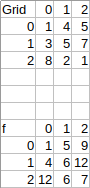
\includegraphics{minimum-path-sum.png}\\
\figcaption{Minimum Path Sum}\label{fig:minimum-path-sum}
\end{center}


\subsubsection{備忘錄法}
\begin{Code}
// LeetCode, Minimum Path Sum
// 備忘錄法
class Solution {
public:
    int minPathSum(vector<vector<int> > &grid) {
        const int m = grid.size();
        const int n = grid[0].size();
        this->f = vector<vector<int> >(m, vector<int>(n, -1));
        return dfs(grid, m-1, n-1);
    }
private:
    vector<vector<int> > f;  // 緩存

    int dfs(const vector<vector<int> > &grid, int x, int y) {
        if (x < 0 || y < 0) return INT_MAX; // 越界,終止條件,注意,不是0

        if (x == 0 && y == 0) return grid[0][0]; // 回到起點,收斂條件

        return min(getOrUpdate(grid, x - 1, y),
                getOrUpdate(grid, x, y - 1)) + grid[x][y];
    }

    int getOrUpdate(const vector<vector<int> > &grid, int x, int y) {
        if (x < 0 || y < 0) return INT_MAX; // 越界,注意,不是0
        if (f[x][y] >= 0) return f[x][y];
        else return f[x][y] = dfs(grid, x, y);
    }
};
\end{Code}


\subsubsection{動規}
\begin{Code}
// LeetCode, Minimum Path Sum
// 二維動規
class Solution {
public:
    int minPathSum(vector<vector<int> > &grid) {
        if (grid.size() == 0) return 0;
        const int m = grid.size();
        const int n = grid[0].size();

        int f[m][n];
        f[0][0] = grid[0][0];
        for (int i = 1; i < m; i++) {
            f[i][0] = f[i - 1][0] + grid[i][0];
        }
        for (int i = 1; i < n; i++) {
            f[0][i] = f[0][i - 1] + grid[0][i];
        }

        for (int i = 1; i < m; i++) {
            for (int j = 1; j < n; j++) {
                f[i][j] = min(f[i - 1][j], f[i][j - 1]) + grid[i][j];
            }
        }
        return f[m - 1][n - 1];
    }
};
\end{Code}


\subsubsection{動規+滾動數組}
\begin{Code}
// LeetCode, Minimum Path Sum
// 二維動規+滾動數組
class Solution {
public:
    int minPathSum(vector<vector<int> > &grid) {
        const int m = grid.size();
        const int n = grid[0].size();

        int f[n];
        fill(f, f+n, INT_MAX); // 初始值是 INT_MAX,因為後面用了min函數。
        f[0] = 0;

        for (int i = 0; i < m; i++) {
            f[0] += grid[i][0];
            for (int j = 1; j < n; j++) {
                // 左邊的f[j],表示更新後的f[j],與公式中的f[i[[j]對應
                // 右邊的f[j],表示老的f[j],與公式中的f[i-1][j]對應
                f[j] = min(f[j - 1], f[j]) + grid[i][j];
            }
        }
        return f[n - 1];
    }
};
\end{Code}

\subsubsection{相關題目}
\begindot
\item Unique Paths, 見 \S \ref{sec:unique-paths}
\item Unique Paths II, 見 \S \ref{sec:unique-paths-ii}
\myenddot


\section{Edit Distance} %%%%%%%%%%%%%%%%%%%%%%%%%%%%%%
\label{sec:edit-distance}


\subsubsection{描述}
Given two words \fn{word1} and \fn{word2}, find the minimum number of steps required to convert \fn{word1} to \fn{word2}. (each operation is counted as 1 step.)

You have the following 3 operations permitted on a word:
\begindot
\item Insert a character
\item Delete a character
\item Replace a character
\myenddot


\subsubsection{分析}
設狀態為\fn{f[i][j]},表示\fn{A[0,i]}和\fn{B[0,j]}之間的最小編輯距離。設\fn{A[0,i]}的形式是\fn{str1c},\fn{B[0,j]}的形式是\fn{str2d},
\begin{enumerate}
\item 如果\fn{c==d},則\fn{f[i][j]=f[i-1][j-1]};
\item 如果\fn{c!=d},
    \begin{enumerate}
        \item 如果將c替換成d,則\fn{f[i][j]=f[i-1][j-1]+1};
        \item 如果在c後面添加一個d,則\fn{f[i][j]=f[i][j-1]+1};
        \item 如果將c刪除,則\fn{f[i][j]=f[i-1][j]+1};
    \end{enumerate}
\end{enumerate}


\begin{center}
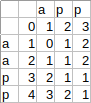
\includegraphics{edit-distance.png}\\
\figcaption{Edit Distance}\label{fig:edit-distance}
\end{center}

\subsubsection{動規}
\begin{Code}
// LeetCode, Edit Distance
// 二維動規,時間複雜度O(n*m),空間複雜度O(n*m)
class Solution {
public:
    int minDistance(const string &word1, const string &word2) {
        const size_t n = word1.size();
        const size_t m = word2.size();
        // 長度為n的字符串,有n+1個隔板
        int f[n + 1][m + 1];
        for (size_t i = 0; i <= n; i++)
            f[i][0] = i;
        for (size_t j = 0; j <= m; j++)
            f[0][j] = j;

        for (size_t i = 1; i <= n; i++) {
            for (size_t j = 1; j <= m; j++) {
                if (word1[i - 1] == word2[j - 1])
                    f[i][j] = f[i - 1][j - 1];
                else {
                    int mn = min(f[i - 1][j], f[i][j - 1]);
                    f[i][j] = 1 + min(f[i - 1][j - 1], mn);
                }
            }
        }
        return f[n][m];
    }
};
\end{Code}


\subsubsection{動規+滾動數組}
\begin{Code}
// LeetCode, Edit Distance
// 二維動規+滾動數組
// 時間複雜度O(n*m),空間複雜度O(n)
class Solution {
public:
    int minDistance(const string &word1, const string &word2) {
        if (word1.length() < word2.length())
            return minDistance(word2, word1);

        int f[word2.length() + 1];
        int upper_left = 0; // 額外用一個變量記錄f[i-1][j-1]

        for (size_t i = 0; i <= word2.size(); ++i)
            f[i] = i;

        for (size_t i = 1; i <= word1.size(); ++i) {
            upper_left = f[0];
            f[0] = i;

            for (size_t j = 1; j <= word2.size(); ++j) {
                int upper = f[j];

                if (word1[i - 1] == word2[j - 1])
                    f[j] = upper_left;
                else
                    f[j] = 1 + min(upper_left, min(f[j], f[j - 1]));

                upper_left = upper;
            }
        }

        return f[word2.length()];
    }
};
\end{Code}


\subsubsection{相關題目}
\begindot
\item 無
\myenddot


\section{Decode Ways} %%%%%%%%%%%%%%%%%%%%%%%%%%%%%%
\label{sec:decode-ways}


\subsubsection{描述}
A message containing letters from \fn{A-Z} is being encoded to numbers using the following mapping:
\begin{Code}
'A' -> 1
'B' -> 2
...
'Z' -> 26
\end{Code}

Given an encoded message containing digits, determine the total number of ways to decode it.

For example,
Given encoded message \fn{"12"}, it could be decoded as \fn{"AB"} (1 2) or \fn{"L"} (12).

The number of ways decoding \fn{"12"} is 2.


\subsubsection{分析}
跟 Climbing Stairs (見 \S \ref{sec:climbing-stairs})很類似,不過多加一些判斷邏輯。


\subsubsection{代碼}
\begin{Code}
// LeetCode, Decode Ways
// 動規,時間複雜度O(n),空間複雜度O(1)
class Solution {
public:
    int numDecodings(const string &s) {
        if (s.empty() || s[0] == '0') return 0;

        int prev = 0;
        int cur = 1;
        // 長度為n的字符串,有 n+1個階梯
        for (size_t i = 1; i <= s.size(); ++i) {
            if (s[i-1] == '0') cur = 0;

            if (i < 2 || !(s[i - 2] == '1' ||
                     (s[i - 2] == '2' && s[i - 1] <= '6')))
                prev = 0;

            int tmp = cur;
            cur = prev + cur;
            prev = tmp;
        }
        return cur;
    }
};
\end{Code}


\subsubsection{相關題目}
\begindot
\item Climbing Stairs, 見 \S \ref{sec:climbing-stairs}
\myenddot


\section{Distinct Subsequences} %%%%%%%%%%%%%%%%%%%%%%%%%%%%%%
\label{sec:distinct-subsequences}


\subsubsection{描述}
Given a string $S$ and a string $T$, count the number of distinct subsequences of $T$ in $S$.

A subsequence of a string is a new string which is formed from the original string by deleting some (can be none) of the characters without disturbing the relative positions of the remaining characters. (ie, \fn{"ACE"} is a subsequence of \fn{"ABCDE"} while \fn{"AEC"} is not).

Here is an example:
$S$ = \fn{"rabbbit"}, $T$ = \fn{"rabbit"}

Return 3.


\subsubsection{分析}
設狀態為$f(i,j)$,表示\fn{T[0,j]}在\fn{S[0,i]}裏出現的次數。首先,無論\fn{S[i]}和\fn{T[j]}是否相等,若不使用\fn{S[i]},則$f(i,j)=f(i-1,j)$;若\fn{S[i]==T[j]},則可以使用\fn{S[i]},此時$f(i,j)=f(i-1,j)+f(i-1, j-1)$。

\begin{center}
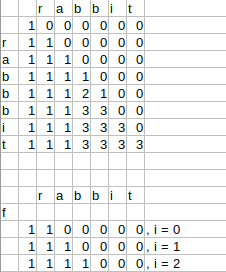
\includegraphics{distinct-subsequences.png}\\
\figcaption{Distinct Subsequences}\label{fig:distinct-subsequences}
\end{center}

\subsubsection{代碼}
\begin{Code}
// LeetCode, Distinct Subsequences
// 二維動規+滾動數組
// 時間複雜度O(m*n),空間複雜度O(n)
class Solution {
public:
    int numDistinct(const string &S, const string &T) {
        vector<int> f(T.size() + 1);
        f[0] = 1;
        for (int i = 0; i < S.size(); ++i) {
            for (int j = T.size() - 1; j >= 0; --j) {
                f[j + 1] += S[i] == T[j] ? f[j] : 0;
            }
        }

        return f[T.size()];
    }
};
\end{Code}


\subsubsection{相關題目}
\begindot
\item 無
\myenddot


\section{Word Break} %%%%%%%%%%%%%%%%%%%%%%%%%%%%%%
\label{sec:word-break}


\subsubsection{描述}
Given a string s and a dictionary of words dict, determine if s can be segmented into a space-separated sequence of one or more dictionary words.

For example, given \\
s = \fn{"leetcode"},\\
dict = \fn{["leet", "code"]}.

Return true because \fn{"leetcode"} can be segmented as \fn{"leet code"}.


\subsubsection{分析}
設狀態為$f(i)$,表示\fn{s[0,i]}是否可以分詞,則狀態轉移方程為
$$
f(i) = any\_of(f(j) \&\& s[j+1,i] \in dict),  0 \leq j < i
$$


\subsubsection{深搜}
\begin{Code}
// LeetCode, Word Break
// 深搜,超時
// 時間複雜度O(2^n),空間複雜度O(n)
class Solution {
public:
    bool wordBreak(string s, unordered_set<string> &dict) {
        return dfs(s, dict, 0, 0);
    }
private:
    static bool dfs(const string &s, unordered_set<string> &dict,
            size_t start, size_t cur) {
        if (cur == s.size()) {
            return dict.find(s.substr(start, cur-start+1)) != dict.end();
        }
        if (dfs(s, dict, start, cur+1)) return true;
        if (dict.find(s.substr(start, cur-start+1)) != dict.end())
            if (dfs(s, dict, cur+1, cur+1)) return true;
        return false;
    }
};
\end{Code}


\subsubsection{動規}
\begin{Code}
// LeetCode, Word Break
// 動規,時間複雜度O(n^2),空間複雜度O(n)
class Solution {
public:
    bool wordBreak(string s, unordered_set<string> &dict) {
        // 長度為n的字符串有n+1個隔板
        vector<bool> f(s.size() + 1, false);
        f[0] = true; // 空字符串
        for (int i = 1; i <= s.size(); ++i) {
            for (int j = i - 1; j >= 0; --j) {
                if (f[j] && dict.find(s.substr(j, i - j)) != dict.end()) {
                    f[i] = true;
                    break;
                }
            }
        }
        return f[s.size()];
    }
};
\end{Code}


\subsubsection{相關題目}
\begindot
\item Word Break II, 見 \S \ref{sec:word-break-ii}
\myenddot


\section{Word Break II} %%%%%%%%%%%%%%%%%%%%%%%%%%%%%%
\label{sec:word-break-ii}


\subsubsection{描述}
Given a string s and a dictionary of words dict, add spaces in s to construct a sentence where each word is a valid dictionary word.

Return all such possible sentences.

For example, given  \\
s = \fn{"catsanddog"}, \\
dict = \fn{["cat", "cats", "and", "sand", "dog"]}.

A solution is \fn{["cats and dog", "cat sand dog"]}.


\subsubsection{分析}
在上一題的基礎上,要返回解本身。


\subsubsection{代碼}
\begin{Code}
// LeetCode, Word Break II
// 動規,時間複雜度O(n^2),空間複雜度O(n^2)
class Solution {
public:
    vector<string> wordBreak(string s, unordered_set<string> &dict) {
        // 長度為n的字符串有n+1個隔板
        vector<bool> f(s.length() + 1, false);
        // prev[i][j]為true,表示s[j, i)是一個合法單詞,可以從j處切開
        // 第一行未用
        vector<vector<bool> > prev(s.length() + 1, vector<bool>(s.length()));
        f[0] = true;
        for (size_t i = 1; i <= s.length(); ++i) {
            for (int j = i - 1; j >= 0; --j) {
                if (f[j] && dict.find(s.substr(j, i - j)) != dict.end()) {
                    f[i] = true;
                    prev[i][j] = true;
                }
            }
        }
        vector<string> result;
        vector<string> path;
        gen_path(s, prev, s.length(), path, result);
        return result;

    }
private:
    // DFS遍歷樹,生成路徑
    void gen_path(const string &s, const vector<vector<bool> > &prev,
            int cur, vector<string> &path, vector<string> &result) {
        if (cur == 0) {
            string tmp;
            for (auto iter = path.crbegin(); iter != path.crend(); ++iter)
                tmp += *iter + " ";
            tmp.erase(tmp.end() - 1);
            result.push_back(tmp);
        }
        for (size_t i = 0; i < s.size(); ++i) {
            if (prev[cur][i]) {
                path.push_back(s.substr(i, cur - i));
                gen_path(s, prev, i, path, result);
                path.pop_back();
            }
        }
    }
};
\end{Code}


\subsubsection{相關題目}
\begindot
\item Word Break, 見 \S \ref{sec:word-break}
\myenddot

\section{Word Break III} %%%%%%%%%%%%%%%%%%%%%%%%%%%%%%
\label{sec:word-break-iii}


\subsubsection{描述}
Given a string s and a dictionary of words dict, add spaces in s to construct a sentence where each word is a valid dictionary word.

Return all such possible sentences.

For example, given  \\
s = \fn{"iamace"}, \\
dict = \fn{["i", "a", "am", "ace"]}.

A solution is \fn{["i am ace"]}.


\subsubsection{分析}
This solution can only return 1 combination.
Reference \myurl{https://www.youtube.com/watch?v=WepWFGxiwRs}


\subsubsection{代碼}
\begin{Code}
// LeetCode, Word Break II
// 動規,時間複雜度O(n^2),空間複雜度O(n^2)
class Solution {
public:
    vector<string> wordBreak(string s, unordered_set<string>& dict)
    {
        vector<string> result;
        if (s.size() == 0) return result;

        vector<vector<int> > f(s.size(), vector<int>(s.size(), -1));
        for (size_t l = 1; l <= s.size(); l++)
        {
            for (size_t i = 0; i < s.size() - l + 1; i++)
            {
                size_t j = i + l - 1;
                string temp = s.substr(i, l);
                if (dict.find(s.substr(i, l)) != dict.end())
                {
                    f[i][j] = i;
                }
                else
                {
                    for (size_t k = i; k < j; k++)
                    {
                        if (f[i][k] != -1 && f[k+1][j] != -1)
                        {
                            f[i][j] = k + 1;
                            break;
                        }
                    }
                }
            }
        }

        if (f[0][s.size() - 1] == -1) return result; // return when no solution

        int i = 0; int j = s.size() - 1;
        while (i < j)
        {
            int k = f[i][j];
            if (i == k)
            {
                result.push_back(s.substr(i, j - i + 1));
                break;
            }
            result.push_back(s.substr(i, k - i));
            i = k;
        }
        return result;
    }
private:
};
\end{Code}


\subsubsection{相關題目}
\begindot
\item Word Break, 見 \S \ref{sec:word-break}
\myenddot
